\documentclass[12pt, titlepage]{article}

\usepackage[normalem]{ulem}
\usepackage{cancel}
\usepackage[a4paper,margin=1in,footskip=0.25in]{geometry}
\usepackage{indentfirst}
\usepackage{xcolor}
\usepackage{tabularx}
\usepackage{booktabs}
\usepackage{hyperref}
\usepackage{listings}
\usepackage{graphicx}
\hypersetup{
    colorlinks,
    citecolor=black,
    filecolor=black,
    linkcolor=black,
    urlcolor=blue
}
\usepackage[round]{natbib}

%%%%%%%%%%%%%
%%% title %%%
%%%%%%%%%%%%%

\title{\textbf{SE 3XA3: Software Requirements Specification}\\Lines Per Minute (lpm)}

\author{Team \#16, Lines Per Minute (lpm)\\
Jay Mody - modyj - 400195508\\
Jessica Lim - limj31 - 400173669\\
Maanav Dalal - dalalm1 - 400178115\\
}

\date{\today}

\begin{document}

\maketitle
\begin{table}[hp]
\caption{Revision History} \label{TblRevisionHistory}
\begin{tabularx}{\textwidth}{llX}
\toprule
\textbf{Date} & \textbf{Developer(s)} & \textbf{Change}\\
\midrule
February 6, 2021 & Jay/Jessica/Maanav & Initial document write-up. \\
February 8, 2021 & Jay/Jessica/Maanav & Document completed \& submitted. \\
March 25, 2021 & Jay/Jessica/Maanav & Edit SRS Document for R1. \\
\bottomrule
\end{tabularx}
\end{table}

\newpage

\tableofcontents
\listoftables
\listoffigures

\newpage

%%%%%%%%%%%%%%%%%%%%%%%
%%% project drivers %%%
%%%%%%%%%%%%%%%%%%%%%%%

This document describes the requirements for lpm (Lines Per Minute).  The template for the Software
Requirements Specification (SRS) is a subset of the Volere
template~\citep{RobertsonAndRobertson2012}.
\section{Project Drivers}

\subsection{The Purpose of the Project}
Typing speed is an increasingly important skill in the digital world. Being a fast typist reduces the friction between transferring thoughts from your mind to your screen. While there are many tools that allow individuals to practice their typing speed for normal text passages, there are few tools to do the same with code. Code, unlike text passages, has a higher frequency of symbols, brackets, and numbers. There are many websites and packages that exist to improve typing speed in typical circumstances, however very few are targeted at the intricacies of coding programs (such as curly braces, camelCase, and semicolons). \\

The goal of the lpm package is to provide a typing tool specialized for code, in a place where you can often find programmers, the command line.

\subsection{The Stakeholders}
\subsubsection{The Client}
In this case the client is the group consisting of the TAs as well as Professor Bokhari - the staff of SFWR ENG 3XA3.
\subsubsection{The Customers}
The customers for lpm are developers or otherwise individuals interested in improving their typing speed in programming contexts. These customers are not paying for the package, as it is open sourced, however they will be using the product, and are deemed customers.
\subsubsection{Other Stakeholders}
Given that it is an open source project, other stakeholders include anyone on the internet who views our project after it is made. This is relevant to three main parties:
\begin{enumerate}
    \item People who look at the source code after our development process for Software Development Principles (i.e. future 3XA3 students)
    \item People who look at the source code after our development process to make a similar or related Python package (in the same way we are using wpm as a foundation to build lpm).
    \item The owners and developers of the open source code that lpm sources for it's code snippet data.
\end{enumerate}
\subsection{Mandated Constraints}
\begin{itemize}
    \item \textbf{Solution constraints}: At completion, the produced system shall be a Python package, and available for download through the pip package manager.
    \item \textbf{Input constraints}: The only device used for input is a keyboard, given that it is a command line application.
    \item \textbf{Space constraints}: The lpm python package shall be no larger than 25 MB of space on the computer's hard drive (using similar Python packages as comparison).
    \item \textbf{Budget constraints}: The lpm package shall cost exactly \$0.00, as all of the developers are unpaid.
    \item \textbf{Schedule constraints}: The lpm package shall be completed on or before April 12th, in accordance with the 3XA3 deadline for the project.
\end{itemize}
\subsection{Naming Conventions and Terminology}
\begin{itemize}
    \item The terms "\textbf{terminal}" and "\textbf{command line}" are used interchangeably.
    \item \textbf{Command line interface} (abbreviated as \textbf{CLI}) is an interface for an application provided through the command line.
    \item \textbf{Command line application}: An application that is delivered using a CLI
    \item \textbf{Typing interface}: The interface that users practice their typing.
    \item \textbf{FR}: Functional requirement.
    \item \textbf{NFR}: Non-functional requirement.
    \item The terms "\textbf{system}" and "\textbf{application}", and "\textbf{product}" all refer to the lpm application this document specifies.
    \item \textbf{pip}: A package manager for python \citep{pip}.
    \item \textbf{PyPI}: The python package index, which serves python packages through the pip tool \citep{pypi}.
\end{itemize}

\subsection{Relevant Facts and Assumptions}
\begin{itemize}
    \item The user should be comfortable using the command line.
    \item The user shall be able to read basic English.
    \item The user shall be running any operating system that can run a Python environment, and running either Python2 or Python3.
    \item The final package will be named lpm assuming that name is available in PyPI (as of the time of writing, it is currently available for use, but has not been claimed).
\end{itemize}

%%%%%%%%%%%%%%%%%%%%%%%%%%%%%%%
%%% functional requirements %%%
%%%%%%%%%%%%%%%%%%%%%%%%%%%%%%%

\section{Functional Requirements}

\subsection{The Scope of the Work and the Product}
Lines Per Minute is a command-line application written in python that's lets individuals practice their typing speed for code. The application is delivered through PyPI as a pip install-able package, and is strictly interfaced via the command line.

\subsubsection{The Context of the Work}
Lines Per Minute is created as the final project for the course SE3XA3 Fall 2021 at McMaster University. The final project for SE3XA3 involves taking a current open source project, and going through the entire software design process to recreate the project with additional features or fixes that improve upon the original project. The project inspiration for lpm is the wpm python package \citep{wpm}. \\

While the wpm package strictly focuses on English text passages, lpm focuses on code snippets. While tools like \href{https://typing.io/}{typing.io} exist, the creators felt that a completely free and non-online solution should exist. As such, wpm provides a perfect starting point for creating a lightweight and free alternative to practicing typing code that can be delivered via the command line. The project was started in January of 2021, and is expected to finish in April of 2021.

\subsubsection{Work Partitioning}
\begin{table}[h]
    \centering
    \begin{tabular}{|c|c|c|c|}
        \hline
        Event Number & Event Name & Input & Output \\
        \hline
        1 & Starting the Typing Interface & Keyboard & Typing Interface\\
        \hline
        2 & Next Code Snippet & Keyboard & Typing Interface\\
        \hline
        3 & Prev Code Snippet & Keyboard & Typing Interface\\
        \hline
        4 & Start the Timer & Keyboard & Typing Interface\\
        \hline
        5 & Stop the Timer & Keyboard & Typing Interface\\
        \hline
        6 & Exit Typing Interface & Keyboard & Return to Command Line\\
        \hline
        7 & Show Stats & Keyboard & Command Line Output\\
        \hline
        8 & Change Settings & Keyboard & Command Line Output\\
        \hline
        9 & Show Help Menu & Keyboard & Command Line Output\\
        \hline
    \end{tabular}
    \caption{Work Partitioning Events}
    \label{tab:workpart}
\end{table}

\begin{table}[h]
    \centering
    \begin{tabular}{| p{0.18\linewidth} | p{0.82\linewidth} |}
        \hline
        Event Number & Summary \\
        \hline
        1 & Using the CLI, the user can start the typing interface with python code snippets via "lpm python". The user can also specify multiple languages to select code snippets from by adding additional arguments "lpm python java javascript".\\
        \hline
        2 & While in the typing interface, the user can use the right arrow key to skip the current snippet and load the next one in the order.\\
        \hline
        3 & While in the typing interface, the user can use the left arrow key to backtrack to load previous code snippet in the order.\\
        \hline
        4 & While in typing interface, the user can start the timer by inputting a keystroke (which will be used as the first input character).\\
        \hline
        5 & While the timer has been started, the user can choose to stop the timer with teh escape key. The timer may be started again using event 4.\\
        \hline
        6 & While \textcolor{red}{in browsing mode (not typing)} \sout{in the typing interface}, the user can press the escape key to quit the typing interface and return to the command line.\\
        \hline
        7 & Using the CLI, the user can show their lifetime stats as command line output via "lpm --stats".\\
        \hline
        8 & Using the CLI, the user can open and modify the json file with the settings via "lpm --settings".\\
        \hline
        9 & Using the CLI, the user can show a help menu via "lpm --help".\\
        \hline
    \end{tabular}
    \caption{Work Partitioning Events Summaries}
    \label{tab:workpartsummary}
\end{table}

\newpage

\subsubsection{Individual Product Use Cases}
%See Figure \ref{fig:usecase} on Page \pageref{fig:usecase}.
\begin{figure}[!htbp]
    \centering
    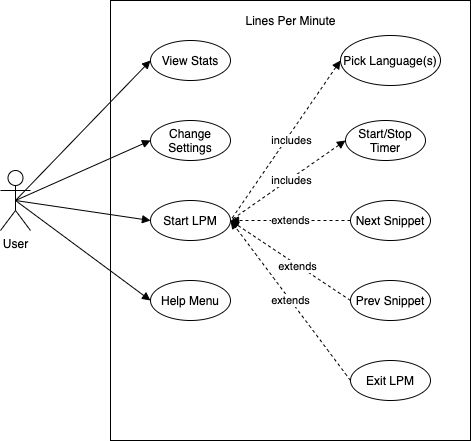
\includegraphics[scale=0.6]{usecase.png}
    \caption{Use Case Diagram for lpm}
    \label{fig:usecase}
\end{figure}

\begin{table}[!htpb]
    \centering
    \begin{tabular}{|p{0.3\linewidth}|p{0.7\linewidth}|}
        \hline
        \textbf{Use Case 1:} & \textbf{View Stats} \\
        \hline
        Related Requirements & FR1, FR4, FR5, FR25, FR26, FR27, FR28\\
        \hline
        Initiating Actor & User\\
        \hline
        Actor's Goal & To display user's typing speed statistics on terminal\\
        \hline
        Participating Actor & lpm system, User\\
        \hline
        Precondition & lpm is installed on commandline\\
        \hline
        Postcondition & User typing speed statistics will be displayed on screen\\
        \hline
        Flow of events & 1. User opens terminal \\
        & 2. User types `lpm --stats` into the terminal \\
        & 3. lpm, wpm and other stats are displayed through the terminal \\
        & 3.1 Alt: If no stats are available, warning is displayed \\
        \hline
    \end{tabular}
    \caption{Use Case 1}
    \label{tab:usecase1}
\end{table}

\bigskip
\begin{table}[!htbp]
    \centering
    \begin{tabular}{|p{0.3\linewidth}|p{0.7\linewidth}|}
        \hline
        \textbf{Use Case 2:} & \textbf{Change Settings} \\
        \hline
        Related Requirements & FR16, FR17, FR18, FR19 \\
        \hline
        Initiating Actor & User\\
        \hline
        Actor's Goal & Change the settings of the lpm settings\\
        \hline
        Participating Actor & lpm system, User\\
        \hline
        Precondition & lpm is installed on commandline\\
        \hline
        Postcondition & lpm main screen settings will be changed to new settings\\
        \hline
        Flow of events & 1. User opens terminal \\
        & 2. User types `lpm --settings` into the terminal \\
        & 3. Settings file will open directly on the terminal \\
        & 4. User can type into the settings to change settings \\
        & 5. User saves settings file \\
        & 6. Settings will be changed to new settings \\
        & 6.1 Alt: User is given warning for invalid settings. Settings are rolled back to previous settings. \\
        \hline
    \end{tabular}
    \caption{Use Case 2}
    \label{tab:usecase2}
\end{table}

\subsection{Functional Requirements}
\subsubsection{Command Line Interface}
\noindent \textbf{FR1}: The CLI shall be avaliable via the command "lpm" inside any directory in a given terminal session (assuming the application has been added to the user's PATH).

\noindent \textbf{FR2}: The CLI shall provide an option to start the typing interface.

\noindent \textbf{FR3}: Upon launch, the CLI shall accept flags that allow the user to select one or more languages for the typing interface.

\noindent \textbf{FR4}: The CLI shall provide an option to view a help menu.

\noindent \textbf{FR5}: The CLI shall provide an option to view lifetime typing statistics.

\noindent \textbf{FR6}: The CLI shall provide an option to change the settings of the program.

\subsubsection{Typing Editor}
\noindent \textbf{FR7}: On startup, the typing interface will randomly generate a code snippet from the specified languages.

\noindent \textbf{FR8}: The typing interface shall display the current code snippet to the user.

\noindent \textbf{FR9}: The typing interface shall display the \textcolor{red}{link} \sout{author and title of the project} where a code snippet was sourced.

\noindent \sout{\textbf{FR10}: The typing interface shall display the session statistics.}

\noindent \textbf{FR11}: The typing interface shall display the current code snippet statistics.

\noindent \textbf{FR12}: The typing interface shall be able to skip ahead to the next code snippet in the list.

\noindent \textbf{FR13}: The typing interface shall be able to backtrack to the previous code snippet in the list.

\noindent \textbf{FR14}: The typing interface shall start the timer and start reading the user's input if they press a non arrow key (the key that is pressed will be considered the first input).

\noindent \textbf{FR15}: The user shall be able to stop the \textcolor{red}{timer when typing a snippet.}

\noindent \textbf{FR16}: The code snippet shall be shown to the user using the TEXT\_COLOR font color.

\noindent \textbf{FR17}: If the user types a correct output for a character, that character shall be indicated as correct with the CORRECT\_COLOR font color.

\noindent \textbf{FR18}: As the user types an incorrect output for a character, that character shall be indicated with the INCORRECT\_COLOR font color.

\noindent \textbf{FR19}: The user shall be able to delete previously typed characters in which case the characters that were deleted are returned to their original TEXT\_COLOR font color.

\noindent \textbf{FR20}: The user shall be able to exit the typing interface.

\subsubsection{Code Snippets}
\noindent \textbf{FR21}: The code snippets shall be shorter than \textcolor{red}{MAX\_LENGTH} \sout{MAX\_SNIPPET\_LENGTH} lines.

\noindent \textbf{FR22}: A line for a code snippet shall not exceed \textcolor{red}{MAX\_COLS} \sout{80} characters.

\noindent \textbf{FR23}: Code snippets should be made available for Python, Java, and JavaScript.

\noindent \textbf{FR24}: Each language shall have a minimum of \textcolor{red}{MIN\_NUM\_SNIPPETS} \sout{20} code snippets.

\subsubsection{Statistics}

\noindent \textbf{FR25}: The application shall track the user's characters per minute speed during a given code snippet, \sout{typing session,} and the entire lifetime history of the application.

\noindent \textbf{FR26}: The application shall track the user's words per minute speed during a given code snippet, \sout{typing session,} and the entire lifetime history of the application.

\noindent \textbf{FR27}: The application shall track the user's lines per minute speed during a given code snippet, \sout{typing session,} and the entire lifetime history of the application.

\noindent \textbf{FR28}: The application shall track the error rate during a given code snippet, \sout{typing session,} and the lifetime entire history of the application. The error rate can be defined as the ratio between correctly typed characters and all characters that were typed.


%%%%%%%%%%%%%%%%%%%%%%%%%%%%%%%%%%%
%%% non-functional requirements %%%
%%%%%%%%%%%%%%%%%%%%%%%%%%%%%%%%%%%

\section{Non-functional Requirements}

\subsection{Look and Feel Requirements}

\noindent \textbf{NFR1}: The typing interface shall respond to a user input within \sout{0.1}{\color{red}10}ms.

\noindent \textbf{NFR2}: The user interface should be visible \sout{in both light and dark terminal backgrounds} {\color{red}regardless of the user's terminal theme}.

\noindent \textbf{NFR3}: The provided theme shall be easy on the eyes and follow the WCAG AA or AAA specification in terms of colour choice.

\noindent \textbf{NFR4}: The code snippets chosen should be diverse, and representative of the languages' syntax.

\noindent \textbf{NFR5}: The entirety of the user interface should fit within a terminal window sized \sout{640x480 pixels or larger, and scale up according on the current terminal window size} {\color{red} greater than MAX\_COLS in width and MAX\_LINES in length}.

\subsection{Usability and Humanity Requirements}

\noindent \textbf{NFR6}: The system's typing interface, as well as its cursor indicator, should be intuitive.

\noindent \textbf{NFR7}: The system shall be easy to use for anyone with basic knowledge of the console.

\noindent \textbf{NFR8}: The instructions will be easily comprehensible by anyone with basic understanding of English

\noindent \textbf{NFR9}: The user will only require the keys on a typical 60\% keyboard to correctly type all given code.

\subsection{Performance Requirements}
\noindent \textbf{NFR10}: When the user loads the package \textcolor{red}{excluding the first time loading}, the time it takes for the package to be ready to accept user input shall not exceed 1 second.

\noindent \textbf{NFR11}: Application should be available 99.999\% (5 nines) of the time. This translates to 5.26 minutes of downtime in a given year, afforded by user updates of python or lpm, as well as unforeseen circumstances in the CI/CD Pipeline.

\subsection{Operational and Environmental Requirements}

\noindent \textbf{NFR12}: The system shall work on \sout{Python 2 and} Python 3{\color{red}.6 and above}.

\noindent \textbf{NFR13}: The system shall work on Linux, macOS, and Windows operating systems.

\noindent \textbf{NFR14}: In terms of computer specs, the package shall run on any computer that is able to run \sout{Python 2 and }Python 3{\color{red}.6+} based on their respective minimum requirements (i.e. if running on Python 3{\color{red}.7}, the user's computer shall at least have Python 3{\color{red}.7}'s minimum requirements to be supported officially by the lpm package).

\noindent \textbf{NFR15}: Application should be installable via the pip package manager.

\subsection{Maintainability and Support Requirements}

\noindent \textbf{NFR16}: Application should be easy to update (via pip).

\noindent \textbf{NFR17}: It should be easy to add additional code snippets.

\subsection{Security Requirements}

\noindent \textbf{NFR18}: External systems shall not have access to the system.

\subsection{Cultural Requirements}

\noindent \textbf{NFR19}: Code snippets that include harmful, vulgar, controversial, political, or offensive content shall not be displayed in lpm

\subsection{Legal Requirements}

\noindent \textbf{NFR20}: Code snippets shall have a valid open source license {\color{red}or the authors of the code snippets have given explicit permission to the developers} to be displayed in lpm.

%%%%%%%%%%%%%%%%%%%%%%
%%% project issues %%%
%%%%%%%%%%%%%%%%%%%%%%

\section{Project Issues}

\subsection{Open Issues}
\begin{itemize}
    \item Finding open-source code snippets that can be used in our product.
    \item Storing large quantities of snippets in an effective and efficient manner.
    \item Creating an aesthetically pleasing interface for individuals with different default console settings.
    \item Supporting multiple programming languages.
\end{itemize}

\subsection{Off-the-Shelf Solutions}
\begin{itemize}
    \item The python package \href{https://github.com/cslarsen/wpm}{wpm} exists as a current command line solution for improving typing speed. However, this application only allows for typing English-language passages.
    \item Current solutions for improving typing speed for coding passages include \href{https://typing.io/}{typing.io}. However, typing.io is a website which involves online internet connection to use.
\end{itemize}

\subsection{New Problems}
Not applicable to our system

\subsection{Tasks}
\begin{tabular}{|c|c|c|}
\hline
Task & Assigned to & Timeline \\
\hline
Requirements Specification & Jessica, Jay, Maanav & Feb 12 2021 \\
\hline
POC - Show output on commmandline & Jessica, Jay, Maanav & Feb 22 2021 \\
\hline
Initial Typing Functionality & Jessica, Jay, Maanav & Mar 5 2021\\
\hline
Test Plan & Jessica, Jay, Maanav & Mar 5 2021\\
\hline
Design Doc Revision & Jessica, Jay, Maanav & Mar 18 2021\\
\hline
Implement all Functional Requirements & Jessica, Jay, Maanav & Mar 18 2021\\
\hline
Fix Bugs & Jessica, Jay, Maanav & Mar 26 2021\\
\hline
Final Product and Presentation & Jessica, Jay, Maanav & Apr 12 2021\\
\hline
\end{tabular}

\subsection{Migration to the New Product}
\begin{itemize}
    \item Functional requirements will each have their own separate branch and Will each be individually implemented into the application.
    \item Every new feature will be created on a separate branch and will include sufficient testing to ensure validity. New code will not be added to the main branch unless it has been tested. This will allow us to keep track of features.
\end{itemize}

\subsection{Risks}
\begin{itemize}
    \item Console keyboard shortcuts may cause issues with our code.
    \item Must ensure that the program can be exited without the key stokes being confused with typing.
\end{itemize}

\subsection{Costs}
There should be no costs associated to this project beyond labour costs.

\subsection{User Documentation and Training}
\begin{itemize}
    \item The lpm application will include a \textit{lpm -h} command that will display a set of instructions for how to use the application, directly within the terminal.
    \item The instructions will also be available online through the PyPI and GitHub.
\end{itemize}

\subsection{Waiting Room}
\begin{itemize}
    \item Product will be available in Java, JavaScript, and other languages.
\end{itemize}

\subsection{Ideas for Solutions}
\begin{itemize}
    \item Created a command line entry-point
    \item Create flags that can be added to lpm command that will let one choose which language to type
    \item Showing updates regarding typing speed after every code passage is completed
\end{itemize}

%%%%%%%%%%%
%%% end %%%
%%%%%%%%%%%

\bibliographystyle{plainnat}

\bibliography{SRS}

\newpage

\section{Appendix}

\subsection{Symbolic Parameters}

\begin{itemize}
    \item TEXT\_COLOR = \textcolor{red}{Terminal Color [252, 235]} \sout{\#FFFFFF}
    \item CORRECT\_COLOR = \textcolor{red}{Terminal Color [243, 235]} \sout{\#00BFFFF}
    \item INCORRECT\_COLOR = \textcolor{red}{Terminal Color [9, 88]}\sout{\#F9BF3B}
    \item \textcolor{red}{MAX\_LENGTH} \sout{MAX\_SNIPPET\_LENGTH} = \textcolor{red}{20} \sout{30}
    \item \textcolor{red}{MAX\_COL} = \textcolor{red}{80}
    \item \textcolor{red}{MIN\_NUM\_SNIPPETS} = \textcolor{red}{10}
\end{itemize}

\end{document}
